\documentclass[12pt]{book}
\usepackage{mathtools}
\usepackage{graphicx}
\usepackage{multicol}


\begin{document}
%\maketitle

%33

	From the previous discussion, the grammar is
\\  	$ S \rightarrow A.B$
\\	  $ A \rightarrow 1A/2A/3A/4A/5A/6A/7A/8A/9A/0/1/2/3/4/5/6/7/8/9$
\\   $	B \rightarrow 0B/1B/2B/3B/4B/5B/6B/7B/8B/9B/1/2/3/4/5/6/7/8/9$


\textbf{\large Example 2.31}Construct the grammar for $WW^R$, where W $\in (a, b)^*$.\\



	\textbf{Solution:} The string W consists of a and b. W can be a null string also. $W^R$ is the reverse string
	of W. \\
	The number of characters in the string $WW^R$ will always be even, except the null string.\\
	So, the string is nothing but an even palindrome of a and b including the null string.
	The grammar is\\
	\[S \rightarrow aSa/bSb/\varepsilon\]
	
	
	
	
	\textbf{\large Example 2.32} Construct the grammar for the language
	
	 $L = a^nb^nc^md^m$ $\quad m, n > 0.$\\

    \textbf{Solution:} The total string can be divided into two parts: (i) string of a and b, where the number of
	a and 
	the number of b are the same and (ii) string of c and d, where the number of c and d is the
	same.\\
	From the start symbol, there will be two non-terminals A and B, where A will generate $a^nb^n$ and B 
	will generate $c^md^m$. In the language set, there will be no null string.
	So the grammar is\\
	\[S \rightarrow AB\]
	\[A \rightarrow aAb/ab\]
	\[B \rightarrow cBd/cd\]
	\textbf{\large Example 2.33} Construct the grammar for the language 
	
	$L = a^nc^md^mb^n$ $\quad m, n > 0.$\\
\textbf{Solution:} In between a and b, there is an equal number of c and d. The number of a and the
	number of 
	b are the same.\\
	So, we have to construct $a^nb^n$ with a non-terminal in between $a^n $ and $ b^n$. From that non-terminal, $c^md^m$
	will be produced.\\
	The grammar constructed according to the previous discussion is
	\[S \rightarrow aSb/aAb\]
	\[A \rightarrow cAd/cd\]      \\
	
	
	\textbf{\Large 2.2 The Chomsky Hierarchy}\\
	The Chomsky hierarchy is an important contribution in the field of formal language and automata theory.  
	In the mid-1950, Noam Chomsky, at the Harvard University, started working on formal
	languages and grammars. He structured a hierarchy of formal languages based on the properties of the
	grammars required to generate the languages. The Chomsky hierarchy drives automata theory one step forward.\\
	Chomsky classified the grammar into four types depending on the production rules.\\
	These are as follows:\\
	\textbf{Type 0:} Type 0 grammar is a phase structure grammar without any restriction. All grammars are type 0 grammar.\\



%34

\textbf{34 $\boldsymbol{\mid}$}Introduction to Automata Theory, Formal Languages and Computation\\
For type 0 grammar, the production rules are in the format of\\
\[\{(L_c)(NT)(R_c)\} \rightarrow \{String\quad of\quad terminal\quad or\quad non-terminals\quad or\quad both\}\]
\[L_c: Left context R_c: Right context NT : Non-terminal \]      \\
\textbf{Type 1:} Type 1 grammar is called context-sensitive grammar.\\
For type 1 grammar, all production rules are context-sensitive if all rules in \textit{P} are of the form

\[\alpha A\beta \rightarrow \alpha \gamma \beta ,\]

where $A \boldsymbol{\varepsilon} NT$ (i.e., A is a single non-terminal), $\boldsymbol{\alpha, \beta \varepsilon (NT \cup \sum)^*}$ (i.e., $\alpha $ and $\beta$ are strings of nonterminals and terminals), and $\boldsymbol{\gamma \varepsilon (NT \cup \sum)}^+$ (i.e., $\boldsymbol{\gamma}$ is a non-empty string of non-terminals and
terminals).\\


\textbf{Type 2:} Type 2 grammar is called context-free grammar. In the LHS of the production, there will no left or right context.\\
For type 2 grammar, all the production rules are in the format of\\
\[(NT) \rightarrow \alpha, where |NT| = 1 and \alpha \varepsilon (NT \cup T)^*\]
\[NT : Non-terminal T : Terminal\]
\begin{multicols}{2}
\textbf{Type 3:} Type 3 grammar is called regular grammar. Here, all the productions will be in the following forms:\\
\begin{center}
A $\rightarrow \alpha \quad  $or A $\rightarrow \alpha B$, where A, B $\varepsilon$ NT and $\alpha \varepsilon $T
\end{center}
The Chomsky classifi cation is called the Chomsky hierarchy. 
This is represented diagrammatically in Fig. 2.7\\
From this diagrammatical representation, we can say that all 
regular grammar is context-free grammar, all context-fre grammar is context-sensitive grammar, and all context-sensitive grammar is unrestricted grammar.\\
The following table shows the different machine formats for different languages.\\
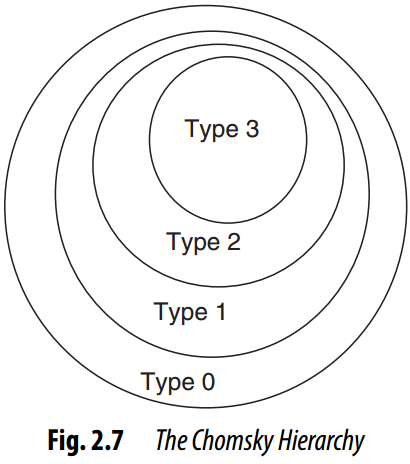
\includegraphics[height=7.5cm,width=6cm]{the chomsky hierarchy.jpg}
\end{multicols}
\begin{center}
\begin{tabular}{ccc}
\hline
 Grammar &  Language & Machine Format\\
 \hline
Type 0 & Unrestricted language & Turing machine\\
Type 1 & Context-sensitive language & Linear bounded automata\\
Type 2 & Context-free language & Push down automata\\
Type 3 & Regular expression & Finite automata\\
\hline
\end{tabular}\\
\end{center}

(Null alphabet is represented by $\varepsilon$. Null string is represented by $\Lambda$. Null set is represented by $\Phi$.)\\
The following are some examples from context-sensitive grammar.\\
\textbf{\large Example 2.34} Construct a grammar for the language $a^nb^nc^n$
, where $n \geq 1$.\\

\textbf{Solution:} We construct it by the following process:\\
1. First, we construct $a^n\alpha^n$.\\
2. Then, from $\alpha^n$ we construct $b^nc^n$. 





%35


\textbf{35 $\boldsymbol{\mid}$}Language and Grammar\\
From $\alpha$, generating $b^nc^n$ is difficult, From $\alpha^n$, $(bc)^n$
can be constructed. But $(bc)^n$ is not equal to bn
$c^n$. \\
Introduce a new non-terminal B.\\
\[S \rightarrow Abc/ABSc\]
\[BA \rightarrow AB\]
\[Bb \rightarrow bb\]
\[A \rightarrow a\]

\textbf{\large Example 2.35} Construct a grammar for the language xx, where\\ $x \in (a, b)^* $\\
\textbf{Solution:}
\[S \rightarrow aAS/bBS\]
\[S \rightarrow aAZ/bBZ\]
\[Aa \rightarrow aA\]
\[Bb \rightarrow bB\]
\[AZ \rightarrow Za\]
\[BZ \rightarrow Zb\]
\[Z \rightarrow \lambda \]

\textbf{\large Example 2.36} Construct a grammar for the language $\{a^nb^nc^nd^n,\\ n\geq1\}$.\\
\textbf{Solution:}
\[S \rightarrow abcd\]
\[S \rightarrow aXbcd\]
\[Xb \rightarrow bX\]
\[Xc \rightarrow bYc\]
\[Yc \rightarrow cY\]
\[Yd \rightarrow Rcdd\]
\[cR \rightarrow Rc\]
\[bR \rightarrow Rb\]
\[aR \rightarrow aaX \mid aa\]
In the Chomsky classifi cation, the different types of grammar and their production rules are
described. 
From the production rules, it is possible to find the highest type of the grammar. The following
are some 
examples of finding the highest type of grammar from the production rules.\\

\textbf{\large Example 2.37} Find the highest type of the following grammar. \\
\[A \rightarrow aA/bB\]
\[B →\rightarrow aB/bB/a/b\]
\textbf{Solution:} The grammar is context-free as the LHS of each production contains only one
non-terminal.
The RHS of each production contains a single terminal or a single terminal followed by nonterminal. 
This matches with regular grammar. So, the grammar is type 3 grammar. \\





%36


\textbf{36 $\boldsymbol{\mid}$}Introduction to Automata Theory, Formal Languages and Computation\\

\textbf{\large Example 2.38} Find the highest type of the following grammar.\\
\[S \rightarrow a/aAS\]
\[A \rightarrow SS/SbA/ba\]
\textbf{Solution:} The grammar is context-free as the LHS of each production contains only one
non-terminal.\\
Now, it is needed to check whether it is regular or not. The RHS of all productions does not contain a single terminal or a single terminal followed by non-terminal. So, the grammar is not regular.Hence, it is type 2 grammar.\\

\textbf{\large Example 2.39} Find the highest type of the following grammar.
\[S →\rightarrow aS/A\]
\[aS \rightarrow aa\]
\[A \rightarrow a\]
\textbf{Solution:} The LHS of the second production rule contains a terminal and a non-terminal (left
context).
So, the grammar is context-sensitive, and hence it is type 1.\\

\begin{center}
\textbf{\Large What We Have Learned So Far}\\
\end{center}
1. The set of rules for constructing a language is called the grammar for that language.\\
2. For every programming language such as C, C++, or Java, there is a grammar.\\
3. Grammar consists of four touples. $G = \{V_N, \sum, P, S\}$, where $V_N$ : set of non-terminals, $\sum$ : set
of terminals, P : set of production rules, S : start symbol.\\
4. Chomsky, a linguist, classifi ed the grammar into four types depending on the productions.The types are type 0, i.e., unrestricted grammar, type 1, i.e., context-sensitive grammar, type 2, i.e., context-free grammar, type 3, i.e., regular grammar.\\
5. For each of the grammar, there is a specifi c language namely unrestricted language, contextsensitive language, context-free language, and regular expression.\\
6. Unrestricted language is accepted by the Turing machine, context-sensitive language isaccepted by linear bounded automata, context-free language is accepted by push down automata, andregular language is accepted by fi nite automata.\\
7. For type 0 grammar, the production rules are in the format of\\ \{$(L_c)(NT)(R_c)$\} $\rightarrow$ \{String of terminals or non-terminals or both\}, where $L_c$: Left context, $R_c$: Right context, and NT: Non-terminal\\
8. For type 1 grammar, all production rules are context-sensitive if all rules in P are of the form $\alpha A\beta \rightarrow \alpha\gamma\beta$, where $A \in NT $(i.e., A is a single non-terminal), $\alpha, \beta \in (NT \cup \sum)^+ $(i.e., $\alpha$ and $\beta$ are strings of non-terminals and terminals), and $\gamma \in (NT \cup \sum)^+ $ (i.e., $\gamma$ is a non-empty string of nonterminals and terminals).\\
9. Type 2 grammar is called context-free grammar. In the LHS of the production, there will be no left or right context. For type 2 grammar, all the production rules are in the format of $(NT) \rightarrow \alpha$, where |NT| = 1 and $\alpha \in (NT \cup T)^*$, NT : Non terminal, and T: Terminal.\\
10. Type 3 grammar is called regular grammar. Here, all the productions will be in the following 
forms: $A \rightarrow \alpha$ or $A \rightarrow \alpha B$, where $A, B \in NT $ and $\alpha \in T.$  



\end{document}